% Created by tikzDevice version 0.12.3 on 2019-12-11 20:53:27
% !TEX encoding = UTF-8 Unicode
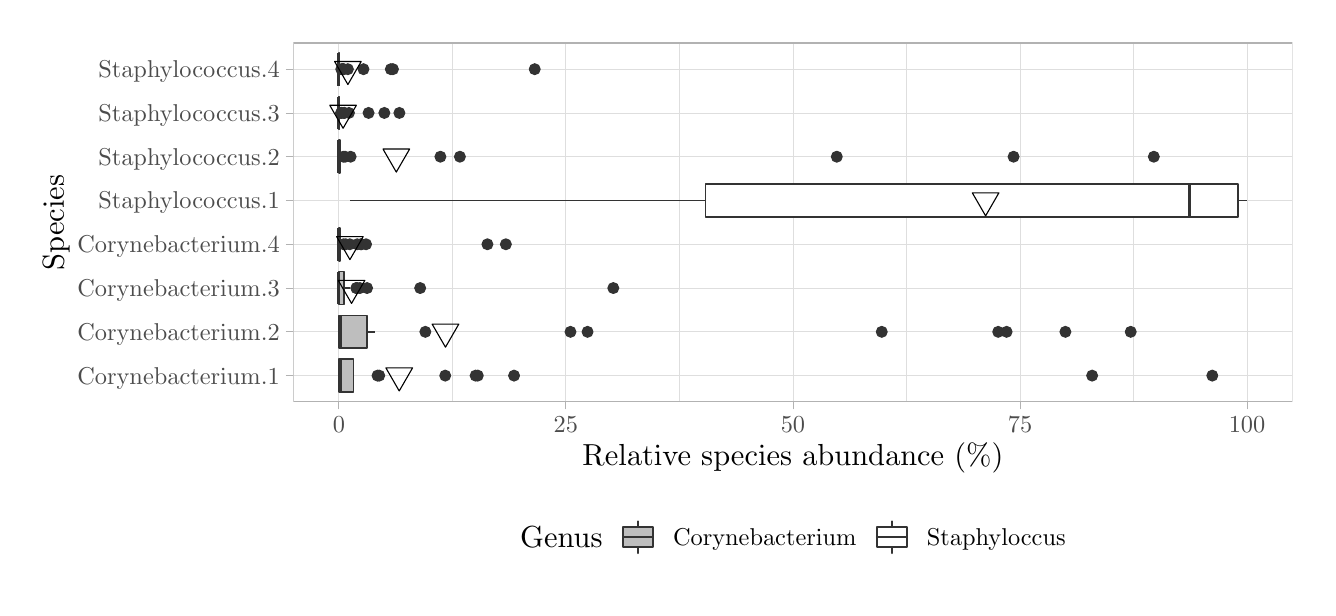
\begin{tikzpicture}[x=1pt,y=1pt]
\definecolor{fillColor}{RGB}{255,255,255}
\path[use as bounding box,fill=fillColor,fill opacity=0.00] (0,0) rectangle (462.53,202.36);
\begin{scope}
\path[clip] (  0.00,  0.00) rectangle (462.53,202.36);
\definecolor{drawColor}{RGB}{255,255,255}
\definecolor{fillColor}{RGB}{255,255,255}

\path[draw=drawColor,line width= 0.6pt,line join=round,line cap=round,fill=fillColor] (  0.00,  0.00) rectangle (462.53,202.36);
\end{scope}
\begin{scope}
\path[clip] ( 96.03, 67.14) rectangle (457.03,196.86);
\definecolor{fillColor}{RGB}{255,255,255}

\path[fill=fillColor] ( 96.03, 67.14) rectangle (457.03,196.86);
\definecolor{drawColor}{gray}{0.87}

\path[draw=drawColor,line width= 0.1pt,line join=round] (153.47, 67.14) --
	(153.47,196.86);

\path[draw=drawColor,line width= 0.1pt,line join=round] (235.51, 67.14) --
	(235.51,196.86);

\path[draw=drawColor,line width= 0.1pt,line join=round] (317.55, 67.14) --
	(317.55,196.86);

\path[draw=drawColor,line width= 0.1pt,line join=round] (399.60, 67.14) --
	(399.60,196.86);

\path[draw=drawColor,line width= 0.3pt,line join=round] ( 96.03, 76.63) --
	(457.03, 76.63);

\path[draw=drawColor,line width= 0.3pt,line join=round] ( 96.03, 92.45) --
	(457.03, 92.45);

\path[draw=drawColor,line width= 0.3pt,line join=round] ( 96.03,108.27) --
	(457.03,108.27);

\path[draw=drawColor,line width= 0.3pt,line join=round] ( 96.03,124.09) --
	(457.03,124.09);

\path[draw=drawColor,line width= 0.3pt,line join=round] ( 96.03,139.91) --
	(457.03,139.91);

\path[draw=drawColor,line width= 0.3pt,line join=round] ( 96.03,155.73) --
	(457.03,155.73);

\path[draw=drawColor,line width= 0.3pt,line join=round] ( 96.03,171.55) --
	(457.03,171.55);

\path[draw=drawColor,line width= 0.3pt,line join=round] ( 96.03,187.36) --
	(457.03,187.36);

\path[draw=drawColor,line width= 0.3pt,line join=round] (112.44, 67.14) --
	(112.44,196.86);

\path[draw=drawColor,line width= 0.3pt,line join=round] (194.49, 67.14) --
	(194.49,196.86);

\path[draw=drawColor,line width= 0.3pt,line join=round] (276.53, 67.14) --
	(276.53,196.86);

\path[draw=drawColor,line width= 0.3pt,line join=round] (358.58, 67.14) --
	(358.58,196.86);

\path[draw=drawColor,line width= 0.3pt,line join=round] (440.62, 67.14) --
	(440.62,196.86);
\definecolor{drawColor}{gray}{0.20}
\definecolor{fillColor}{gray}{0.20}

\path[draw=drawColor,line width= 0.4pt,line join=round,line cap=round,fill=fillColor] (127.04, 76.63) circle (  1.96);

\path[draw=drawColor,line width= 0.4pt,line join=round,line cap=round,fill=fillColor] (126.42, 76.63) circle (  1.96);

\path[draw=drawColor,line width= 0.4pt,line join=round,line cap=round,fill=fillColor] (150.88, 76.63) circle (  1.96);

\path[draw=drawColor,line width= 0.4pt,line join=round,line cap=round,fill=fillColor] (175.75, 76.63) circle (  1.96);

\path[draw=drawColor,line width= 0.4pt,line join=round,line cap=round,fill=fillColor] (162.65, 76.63) circle (  1.96);

\path[draw=drawColor,line width= 0.4pt,line join=round,line cap=round,fill=fillColor] (161.86, 76.63) circle (  1.96);

\path[draw=drawColor,line width= 0.4pt,line join=round,line cap=round,fill=fillColor] (428.06, 76.63) circle (  1.96);

\path[draw=drawColor,line width= 0.4pt,line join=round,line cap=round,fill=fillColor] (384.64, 76.63) circle (  1.96);

\path[draw=drawColor,line width= 0.6pt,line join=round] (117.72, 76.63) -- (118.08, 76.63);

\path[draw=drawColor,line width= 0.6pt,line join=round] (112.44, 76.63) -- (112.44, 76.63);
\definecolor{fillColor}{RGB}{190,190,190}

\path[draw=drawColor,line width= 0.6pt,line join=round,line cap=round,fill=fillColor] (117.72, 70.70) --
	(112.44, 70.70) --
	(112.44, 82.56) --
	(117.72, 82.56) --
	(117.72, 70.70) --
	cycle;

\path[draw=drawColor,line width= 1.1pt,line join=round] (113.09, 70.70) -- (113.09, 82.56);
\definecolor{fillColor}{gray}{0.20}

\path[draw=drawColor,line width= 0.4pt,line join=round,line cap=round,fill=fillColor] (350.69, 92.45) circle (  1.96);

\path[draw=drawColor,line width= 0.4pt,line join=round,line cap=round,fill=fillColor] (374.98, 92.45) circle (  1.96);

\path[draw=drawColor,line width= 0.4pt,line join=round,line cap=round,fill=fillColor] (196.14, 92.45) circle (  1.96);

\path[draw=drawColor,line width= 0.4pt,line join=round,line cap=round,fill=fillColor] (353.73, 92.45) circle (  1.96);

\path[draw=drawColor,line width= 0.4pt,line join=round,line cap=round,fill=fillColor] (143.70, 92.45) circle (  1.96);

\path[draw=drawColor,line width= 0.4pt,line join=round,line cap=round,fill=fillColor] (202.31, 92.45) circle (  1.96);

\path[draw=drawColor,line width= 0.4pt,line join=round,line cap=round,fill=fillColor] (398.58, 92.45) circle (  1.96);

\path[draw=drawColor,line width= 0.4pt,line join=round,line cap=round,fill=fillColor] (308.62, 92.45) circle (  1.96);

\path[draw=drawColor,line width= 0.6pt,line join=round] (122.51, 92.45) -- (125.55, 92.45);

\path[draw=drawColor,line width= 0.6pt,line join=round] (112.44, 92.45) -- (112.44, 92.45);
\definecolor{fillColor}{RGB}{190,190,190}

\path[draw=drawColor,line width= 0.6pt,line join=round,line cap=round,fill=fillColor] (122.51, 86.52) --
	(112.44, 86.52) --
	(112.44, 98.38) --
	(122.51, 98.38) --
	(122.51, 86.52) --
	cycle;

\path[draw=drawColor,line width= 1.1pt,line join=round] (113.10, 86.52) -- (113.10, 98.38);
\definecolor{fillColor}{gray}{0.20}

\path[draw=drawColor,line width= 0.4pt,line join=round,line cap=round,fill=fillColor] (211.62,108.27) circle (  1.96);

\path[draw=drawColor,line width= 0.4pt,line join=round,line cap=round,fill=fillColor] (118.77,108.27) circle (  1.96);

\path[draw=drawColor,line width= 0.4pt,line join=round,line cap=round,fill=fillColor] (118.98,108.27) circle (  1.96);

\path[draw=drawColor,line width= 0.4pt,line join=round,line cap=round,fill=fillColor] (141.83,108.27) circle (  1.96);

\path[draw=drawColor,line width= 0.4pt,line join=round,line cap=round,fill=fillColor] (122.64,108.27) circle (  1.96);

\path[draw=drawColor,line width= 0.4pt,line join=round,line cap=round,fill=fillColor] (118.85,108.27) circle (  1.96);

\path[draw=drawColor,line width= 0.4pt,line join=round,line cap=round,fill=fillColor] (120.07,108.27) circle (  1.96);

\path[draw=drawColor,line width= 0.6pt,line join=round] (114.22,108.27) -- (116.54,108.27);

\path[draw=drawColor,line width= 0.6pt,line join=round] (112.44,108.27) -- (112.44,108.27);
\definecolor{fillColor}{RGB}{190,190,190}

\path[draw=drawColor,line width= 0.6pt,line join=round,line cap=round,fill=fillColor] (114.22,102.34) --
	(112.44,102.34) --
	(112.44,114.20) --
	(114.22,114.20) --
	(114.22,102.34) --
	cycle;

\path[draw=drawColor,line width= 1.1pt,line join=round] (112.44,102.34) -- (112.44,114.20);
\definecolor{fillColor}{gray}{0.20}

\path[draw=drawColor,line width= 0.4pt,line join=round,line cap=round,fill=fillColor] (172.79,124.09) circle (  1.96);

\path[draw=drawColor,line width= 0.4pt,line join=round,line cap=round,fill=fillColor] (114.92,124.09) circle (  1.96);

\path[draw=drawColor,line width= 0.4pt,line join=round,line cap=round,fill=fillColor] (120.37,124.09) circle (  1.96);

\path[draw=drawColor,line width= 0.4pt,line join=round,line cap=round,fill=fillColor] (166.13,124.09) circle (  1.96);

\path[draw=drawColor,line width= 0.4pt,line join=round,line cap=round,fill=fillColor] (116.40,124.09) circle (  1.96);

\path[draw=drawColor,line width= 0.4pt,line join=round,line cap=round,fill=fillColor] (120.60,124.09) circle (  1.96);

\path[draw=drawColor,line width= 0.4pt,line join=round,line cap=round,fill=fillColor] (122.27,124.09) circle (  1.96);

\path[draw=drawColor,line width= 0.4pt,line join=round,line cap=round,fill=fillColor] (114.11,124.09) circle (  1.96);

\path[draw=drawColor,line width= 0.4pt,line join=round,line cap=round,fill=fillColor] (119.07,124.09) circle (  1.96);

\path[draw=drawColor,line width= 0.6pt,line join=round] (112.93,124.09) -- (113.00,124.09);

\path[draw=drawColor,line width= 0.6pt,line join=round] (112.44,124.09) -- (112.44,124.09);
\definecolor{fillColor}{RGB}{190,190,190}

\path[draw=drawColor,line width= 0.6pt,line join=round,line cap=round,fill=fillColor] (112.93,118.16) --
	(112.44,118.16) --
	(112.44,130.02) --
	(112.93,130.02) --
	(112.93,118.16) --
	cycle;

\path[draw=drawColor,line width= 1.1pt,line join=round] (112.44,118.16) -- (112.44,130.02);

\path[draw=drawColor,line width= 0.6pt,line join=round] (437.41,139.91) -- (440.62,139.91);

\path[draw=drawColor,line width= 0.6pt,line join=round] (244.88,139.91) -- (116.39,139.91);
\definecolor{fillColor}{RGB}{255,255,255}

\path[draw=drawColor,line width= 0.6pt,line join=round,line cap=round,fill=fillColor] (437.41,133.98) --
	(244.88,133.98) --
	(244.88,145.84) --
	(437.41,145.84) --
	(437.41,133.98) --
	cycle;

\path[draw=drawColor,line width= 1.1pt,line join=round] (419.86,133.98) -- (419.86,145.84);
\definecolor{fillColor}{gray}{0.20}

\path[draw=drawColor,line width= 0.4pt,line join=round,line cap=round,fill=fillColor] (156.18,155.73) circle (  1.96);

\path[draw=drawColor,line width= 0.4pt,line join=round,line cap=round,fill=fillColor] (292.37,155.73) circle (  1.96);

\path[draw=drawColor,line width= 0.4pt,line join=round,line cap=round,fill=fillColor] (149.14,155.73) circle (  1.96);

\path[draw=drawColor,line width= 0.4pt,line join=round,line cap=round,fill=fillColor] (114.06,155.73) circle (  1.96);

\path[draw=drawColor,line width= 0.4pt,line join=round,line cap=round,fill=fillColor] (116.69,155.73) circle (  1.96);

\path[draw=drawColor,line width= 0.4pt,line join=round,line cap=round,fill=fillColor] (114.71,155.73) circle (  1.96);

\path[draw=drawColor,line width= 0.4pt,line join=round,line cap=round,fill=fillColor] (356.25,155.73) circle (  1.96);

\path[draw=drawColor,line width= 0.4pt,line join=round,line cap=round,fill=fillColor] (406.93,155.73) circle (  1.96);

\path[draw=drawColor,line width= 0.6pt,line join=round] (112.97,155.73) -- (113.69,155.73);

\path[draw=drawColor,line width= 0.6pt,line join=round] (112.44,155.73) -- (112.44,155.73);
\definecolor{fillColor}{RGB}{255,255,255}

\path[draw=drawColor,line width= 0.6pt,line join=round,line cap=round,fill=fillColor] (112.97,149.79) --
	(112.44,149.79) --
	(112.44,161.66) --
	(112.97,161.66) --
	(112.97,149.79) --
	cycle;

\path[draw=drawColor,line width= 1.1pt,line join=round] (112.44,149.79) -- (112.44,161.66);
\definecolor{fillColor}{gray}{0.20}

\path[draw=drawColor,line width= 0.4pt,line join=round,line cap=round,fill=fillColor] (113.41,171.55) circle (  1.96);

\path[draw=drawColor,line width= 0.4pt,line join=round,line cap=round,fill=fillColor] (114.42,171.55) circle (  1.96);

\path[draw=drawColor,line width= 0.4pt,line join=round,line cap=round,fill=fillColor] (128.88,171.55) circle (  1.96);

\path[draw=drawColor,line width= 0.4pt,line join=round,line cap=round,fill=fillColor] (134.32,171.55) circle (  1.96);

\path[draw=drawColor,line width= 0.4pt,line join=round,line cap=round,fill=fillColor] (123.18,171.55) circle (  1.96);

\path[draw=drawColor,line width= 0.4pt,line join=round,line cap=round,fill=fillColor] (114.36,171.55) circle (  1.96);

\path[draw=drawColor,line width= 0.4pt,line join=round,line cap=round,fill=fillColor] (113.21,171.55) circle (  1.96);

\path[draw=drawColor,line width= 0.4pt,line join=round,line cap=round,fill=fillColor] (116.09,171.55) circle (  1.96);

\path[draw=drawColor,line width= 0.6pt,line join=round] (112.66,171.55) -- (112.80,171.55);

\path[draw=drawColor,line width= 0.6pt,line join=round] (112.44,171.55) -- (112.44,171.55);
\definecolor{fillColor}{RGB}{255,255,255}

\path[draw=drawColor,line width= 0.6pt,line join=round,line cap=round,fill=fillColor] (112.66,165.61) --
	(112.44,165.61) --
	(112.44,177.48) --
	(112.66,177.48) --
	(112.66,165.61) --
	cycle;

\path[draw=drawColor,line width= 1.1pt,line join=round] (112.44,165.61) -- (112.44,177.48);
\definecolor{fillColor}{gray}{0.20}

\path[draw=drawColor,line width= 0.4pt,line join=round,line cap=round,fill=fillColor] (114.05,187.36) circle (  1.96);

\path[draw=drawColor,line width= 0.4pt,line join=round,line cap=round,fill=fillColor] (131.22,187.36) circle (  1.96);

\path[draw=drawColor,line width= 0.4pt,line join=round,line cap=round,fill=fillColor] (183.22,187.36) circle (  1.96);

\path[draw=drawColor,line width= 0.4pt,line join=round,line cap=round,fill=fillColor] (114.18,187.36) circle (  1.96);

\path[draw=drawColor,line width= 0.4pt,line join=round,line cap=round,fill=fillColor] (131.99,187.36) circle (  1.96);

\path[draw=drawColor,line width= 0.4pt,line join=round,line cap=round,fill=fillColor] (113.82,187.36) circle (  1.96);

\path[draw=drawColor,line width= 0.4pt,line join=round,line cap=round,fill=fillColor] (121.34,187.36) circle (  1.96);

\path[draw=drawColor,line width= 0.4pt,line join=round,line cap=round,fill=fillColor] (113.31,187.36) circle (  1.96);

\path[draw=drawColor,line width= 0.4pt,line join=round,line cap=round,fill=fillColor] (115.71,187.36) circle (  1.96);

\path[draw=drawColor,line width= 0.6pt,line join=round] (112.73,187.36) -- (112.79,187.36);

\path[draw=drawColor,line width= 0.6pt,line join=round] (112.44,187.36) -- (112.44,187.36);
\definecolor{fillColor}{RGB}{255,255,255}

\path[draw=drawColor,line width= 0.6pt,line join=round,line cap=round,fill=fillColor] (112.73,181.43) --
	(112.44,181.43) --
	(112.44,193.30) --
	(112.73,193.30) --
	(112.73,181.43) --
	cycle;

\path[draw=drawColor,line width= 1.1pt,line join=round] (112.44,181.43) -- (112.44,193.30);
\definecolor{drawColor}{RGB}{0,0,0}

\path[draw=drawColor,line width= 0.4pt,line join=round,line cap=round] (134.26, 71.08) --
	(139.07, 79.41) --
	(129.45, 79.41) --
	(134.26, 71.08);

\path[draw=drawColor,line width= 0.4pt,line join=round,line cap=round] (150.97, 86.90) --
	(155.78, 95.23) --
	(146.16, 95.23) --
	(150.97, 86.90);

\path[draw=drawColor,line width= 0.4pt,line join=round,line cap=round] (117.03,102.72) --
	(121.83,111.04) --
	(112.22,111.04) --
	(117.03,102.72);

\path[draw=drawColor,line width= 0.4pt,line join=round,line cap=round] (116.44,118.54) --
	(121.25,126.86) --
	(111.64,126.86) --
	(116.44,118.54);

\path[draw=drawColor,line width= 0.4pt,line join=round,line cap=round] (346.15,134.36) --
	(350.95,142.68) --
	(341.34,142.68) --
	(346.15,134.36);

\path[draw=drawColor,line width= 0.4pt,line join=round,line cap=round] (133.20,150.18) --
	(138.01,158.50) --
	(128.39,158.50) --
	(133.20,150.18);

\path[draw=drawColor,line width= 0.4pt,line join=round,line cap=round] (113.97,166.00) --
	(118.77,174.32) --
	(109.16,174.32) --
	(113.97,166.00);

\path[draw=drawColor,line width= 0.4pt,line join=round,line cap=round] (115.71,181.81) --
	(120.52,190.14) --
	(110.91,190.14) --
	(115.71,181.81);
\definecolor{drawColor}{gray}{0.70}

\path[draw=drawColor,line width= 0.6pt,line join=round,line cap=round] ( 96.03, 67.14) rectangle (457.03,196.86);
\end{scope}
\begin{scope}
\path[clip] (  0.00,  0.00) rectangle (462.53,202.36);
\definecolor{drawColor}{gray}{0.30}

\node[text=drawColor,anchor=base east,inner sep=0pt, outer sep=0pt, scale=  0.88] at ( 91.08, 73.60) {Corynebacterium.1};

\node[text=drawColor,anchor=base east,inner sep=0pt, outer sep=0pt, scale=  0.88] at ( 91.08, 89.42) {Corynebacterium.2};

\node[text=drawColor,anchor=base east,inner sep=0pt, outer sep=0pt, scale=  0.88] at ( 91.08,105.24) {Corynebacterium.3};

\node[text=drawColor,anchor=base east,inner sep=0pt, outer sep=0pt, scale=  0.88] at ( 91.08,121.06) {Corynebacterium.4};

\node[text=drawColor,anchor=base east,inner sep=0pt, outer sep=0pt, scale=  0.88] at ( 91.08,136.88) {Staphylococcus.1};

\node[text=drawColor,anchor=base east,inner sep=0pt, outer sep=0pt, scale=  0.88] at ( 91.08,152.70) {Staphylococcus.2};

\node[text=drawColor,anchor=base east,inner sep=0pt, outer sep=0pt, scale=  0.88] at ( 91.08,168.52) {Staphylococcus.3};

\node[text=drawColor,anchor=base east,inner sep=0pt, outer sep=0pt, scale=  0.88] at ( 91.08,184.33) {Staphylococcus.4};
\end{scope}
\begin{scope}
\path[clip] (  0.00,  0.00) rectangle (462.53,202.36);
\definecolor{drawColor}{gray}{0.70}

\path[draw=drawColor,line width= 0.3pt,line join=round] ( 93.28, 76.63) --
	( 96.03, 76.63);

\path[draw=drawColor,line width= 0.3pt,line join=round] ( 93.28, 92.45) --
	( 96.03, 92.45);

\path[draw=drawColor,line width= 0.3pt,line join=round] ( 93.28,108.27) --
	( 96.03,108.27);

\path[draw=drawColor,line width= 0.3pt,line join=round] ( 93.28,124.09) --
	( 96.03,124.09);

\path[draw=drawColor,line width= 0.3pt,line join=round] ( 93.28,139.91) --
	( 96.03,139.91);

\path[draw=drawColor,line width= 0.3pt,line join=round] ( 93.28,155.73) --
	( 96.03,155.73);

\path[draw=drawColor,line width= 0.3pt,line join=round] ( 93.28,171.55) --
	( 96.03,171.55);

\path[draw=drawColor,line width= 0.3pt,line join=round] ( 93.28,187.36) --
	( 96.03,187.36);
\end{scope}
\begin{scope}
\path[clip] (  0.00,  0.00) rectangle (462.53,202.36);
\definecolor{drawColor}{gray}{0.70}

\path[draw=drawColor,line width= 0.3pt,line join=round] (112.44, 64.39) --
	(112.44, 67.14);

\path[draw=drawColor,line width= 0.3pt,line join=round] (194.49, 64.39) --
	(194.49, 67.14);

\path[draw=drawColor,line width= 0.3pt,line join=round] (276.53, 64.39) --
	(276.53, 67.14);

\path[draw=drawColor,line width= 0.3pt,line join=round] (358.58, 64.39) --
	(358.58, 67.14);

\path[draw=drawColor,line width= 0.3pt,line join=round] (440.62, 64.39) --
	(440.62, 67.14);
\end{scope}
\begin{scope}
\path[clip] (  0.00,  0.00) rectangle (462.53,202.36);
\definecolor{drawColor}{gray}{0.30}

\node[text=drawColor,anchor=base,inner sep=0pt, outer sep=0pt, scale=  0.88] at (112.44, 56.13) {0};

\node[text=drawColor,anchor=base,inner sep=0pt, outer sep=0pt, scale=  0.88] at (194.49, 56.13) {25};

\node[text=drawColor,anchor=base,inner sep=0pt, outer sep=0pt, scale=  0.88] at (276.53, 56.13) {50};

\node[text=drawColor,anchor=base,inner sep=0pt, outer sep=0pt, scale=  0.88] at (358.58, 56.13) {75};

\node[text=drawColor,anchor=base,inner sep=0pt, outer sep=0pt, scale=  0.88] at (440.62, 56.13) {100};
\end{scope}
\begin{scope}
\path[clip] (  0.00,  0.00) rectangle (462.53,202.36);
\definecolor{drawColor}{RGB}{0,0,0}

\node[text=drawColor,anchor=base,inner sep=0pt, outer sep=0pt, scale=  1.10] at (276.53, 44.09) {Relative species abundance (\%)};
\end{scope}
\begin{scope}
\path[clip] (  0.00,  0.00) rectangle (462.53,202.36);
\definecolor{drawColor}{RGB}{0,0,0}

\node[text=drawColor,rotate= 90.00,anchor=base,inner sep=0pt, outer sep=0pt, scale=  1.10] at ( 13.08,132.00) {Species};
\end{scope}
\begin{scope}
\path[clip] (  0.00,  0.00) rectangle (462.53,202.36);
\definecolor{fillColor}{RGB}{255,255,255}

\path[fill=fillColor] (172.48,  5.50) rectangle (380.58, 30.95);
\end{scope}
\begin{scope}
\path[clip] (  0.00,  0.00) rectangle (462.53,202.36);
\definecolor{drawColor}{RGB}{0,0,0}

\node[text=drawColor,anchor=base west,inner sep=0pt, outer sep=0pt, scale=  1.10] at (177.98, 14.44) {Genus};
\end{scope}
\begin{scope}
\path[clip] (  0.00,  0.00) rectangle (462.53,202.36);
\definecolor{fillColor}{RGB}{255,255,255}

\path[fill=fillColor] (213.25, 11.00) rectangle (227.70, 25.45);
\end{scope}
\begin{scope}
\path[clip] (  0.00,  0.00) rectangle (462.53,202.36);
\definecolor{drawColor}{gray}{0.20}

\path[draw=drawColor,line width= 0.6pt,line join=round,line cap=round] (220.48, 12.45) --
	(220.48, 14.61);

\path[draw=drawColor,line width= 0.6pt,line join=round,line cap=round] (220.48, 21.84) --
	(220.48, 24.01);
\definecolor{fillColor}{RGB}{190,190,190}

\path[draw=drawColor,line width= 0.6pt,line join=round,line cap=round,fill=fillColor] (215.06, 14.61) rectangle (225.90, 21.84);

\path[draw=drawColor,line width= 0.6pt,line join=round,line cap=round] (215.06, 18.23) --
	(225.90, 18.23);
\end{scope}
\begin{scope}
\path[clip] (  0.00,  0.00) rectangle (462.53,202.36);
\definecolor{fillColor}{RGB}{255,255,255}

\path[fill=fillColor] (304.98, 11.00) rectangle (319.43, 25.45);
\end{scope}
\begin{scope}
\path[clip] (  0.00,  0.00) rectangle (462.53,202.36);
\definecolor{drawColor}{gray}{0.20}

\path[draw=drawColor,line width= 0.6pt,line join=round,line cap=round] (312.21, 12.45) --
	(312.21, 14.61);

\path[draw=drawColor,line width= 0.6pt,line join=round,line cap=round] (312.21, 21.84) --
	(312.21, 24.01);
\definecolor{fillColor}{RGB}{255,255,255}

\path[draw=drawColor,line width= 0.6pt,line join=round,line cap=round,fill=fillColor] (306.79, 14.61) rectangle (317.63, 21.84);

\path[draw=drawColor,line width= 0.6pt,line join=round,line cap=round] (306.79, 18.23) --
	(317.63, 18.23);
\end{scope}
\begin{scope}
\path[clip] (  0.00,  0.00) rectangle (462.53,202.36);
\definecolor{drawColor}{RGB}{0,0,0}

\node[text=drawColor,anchor=base west,inner sep=0pt, outer sep=0pt, scale=  0.88] at (233.20, 15.20) {Corynebacterium};
\end{scope}
\begin{scope}
\path[clip] (  0.00,  0.00) rectangle (462.53,202.36);
\definecolor{drawColor}{RGB}{0,0,0}

\node[text=drawColor,anchor=base west,inner sep=0pt, outer sep=0pt, scale=  0.88] at (324.93, 15.20) {Staphyloccus};
\end{scope}
\end{tikzpicture}
